\chapter{Optimisations}
    Cette partie est consacrée à l'étude et à l'implémentation de quelques améliorations possibles pour l'algorithme $\rho$ de Pollard.

    \section{r-adding walks}
      \subsection{Théorie}
      L'algorithme $\rho$ de Pollard original ne permet pas d'atteindre les performances d'une marche aléatoire. D'autres méthodes plus performantes ont donc été développées. Parmi elles, la variante des r-adding walks, que nous allons étudier à présent.

      Comme pour la méthode originale, il faut commencer par partitionner le groupe $G$ en sous-ensembles d'environ la même taille. On choisit donc un entier naturel $3 \leq r \leq 100$ et on trouve $r$ sous-ensembles $(T_i)_{i \in \{0,\cdots,r-1\}}$ de tailles à peu près équivalentes. On obtient ainsi $G = \bigcup\limits_{i=0}^{r-1} T_i$. On définit la fonction d'indexation $s$ comme suit~:

      \begin{center}
        $\begin{array}{lrcl}
        s : & G & \longrightarrow & \{0,1,\cdots,r-1\} \\
            & x & \longmapsto & s \text{ si } x \in T_s
        \end{array}$
      \end{center}

      Pour chacun des nombres $s \in \{0,\cdots,r-1\}$, on choisit aléatoirement deux entiers $m_s$ et $n_s$ dans $\mathbb{Z}/q\mathbb{Z}$ et on pose $M_s = g^{m_s} \cdot h^{n_s}$. Enfin, on définit la fonction d'itération $f$ comme $f(x) = x \cdot M_{s(x)}$ et la suite $(x_i)_{i \ge 0}$ par $x_0 = 1$ et $x_{i+1} = f(x_i)$. A présent, montrons que $f$ permet le traçage des exposants par rapport à $g$ et $h$.

      Il faut trouver deux suites $(a_i)_{i \ge 0}$ et $(b_i)_{i \ge 0}$ telles que $x_i = g^{a_i} \cdot h^{b_i}$ pour tout $i$. Posons :

      \begin{align*}
        \begin{cases}
          a_0 = 0 \\
          a_{i+1} = a_i + m_{s(x_i)}
        \end{cases}
      \end{align*}

      \begin{align*}
        \begin{cases}
          b_0 = 0 \\
          b_{i+1} = b_i + n_{s(x_i)}
        \end{cases}
      \end{align*}

      Comme pour la méthode originale de l'algorithme $\rho$ de Pollard, dans quelques rares cas cette fonction d'itération ne permet pas de détecter une collision. Il suffit alors de prendre les entiers $a_0$ et $b_0$ aléatoirement dans l'intervalle $\mathopen{[}1,q-1\mathclose{]}$ et de poser $x_0 = g^{a_0} \cdot h^{b_0}$. On exécute ensuite l'algorithme normalement.

      Montrons par récurrence que ces deux suites conviennent.

        \subsubsection*{Initialisation}
        Dans le cas général, par définition, $x_0 = 1$, $a_0 = 0$ et $b_0 = 0$. On a donc~:

        \begin{align*}
              g^{a_0} \cdot h^{b_0} &= g^{0} \cdot h^{0} \\
                                    &= 1 \cdot 1 \\
                                    &= x_0
        \end{align*}

        Dans les quelques rares cas où $a_0$ et $b_0$ sont choisis aléatoirement dans $\mathopen{[}1,q-1\mathclose{]}$, on a $x_0 = g^{a_0} \cdot h^{b_0}$ par définition.

        La relation est donc vraie au rang $0$.

        \subsubsection*{Hérédité}
        On suppose que la relation est vérifiée pour un $k \in \mathbb{N}$, c'est-à-dire $x_k = g^{a_k} \cdot h^{b_k}$. Montrons que l'on a $x_{k+1} = g^{a_{k+1}} \cdot h^{b_{k+1}}$.

        Par définition $x_{k+1} = f(x_k) = x_k \cdot M_{s(x_k)}$. Par hypothèse de récurrence, on a donc~:

        \begin{align*}
           x_{k+1} &= g^{a_k} \cdot h^{b_k} \cdot g^{m_{s(x_k)}} \cdot h^{n_{s(x_k)}} \\
                   &= g^{a_k + m_{s(x_k)}} \cdot h^{b_k + n_{s(x_k)}} \\
                   &=g^{a_{k+1}} \cdot h^{b_{k+1}}
        \end{align*}

        \subsubsection*{Conclusion}
        On a montré que la relation est vraie pour $i = 0$, et que si elle est vérifiée au rang $k$, elle l'est aussi au rang $k + 1$. Donc pour tout $i \in \mathbb{N}$, $x_i = g^{a_i} \cdot h^{b_i}$.

      % TODO
      \subsection{Implémentation}
      \subsection{Résultats}
      En utilisant le protocole défini dans le chapitre précédent (\ref{chapter2:protocole_de_mesure}), nous avons mesuré les performances de notre implémentation de la méthode "r-adding walks".

      \begin{figure}
        \center{}
        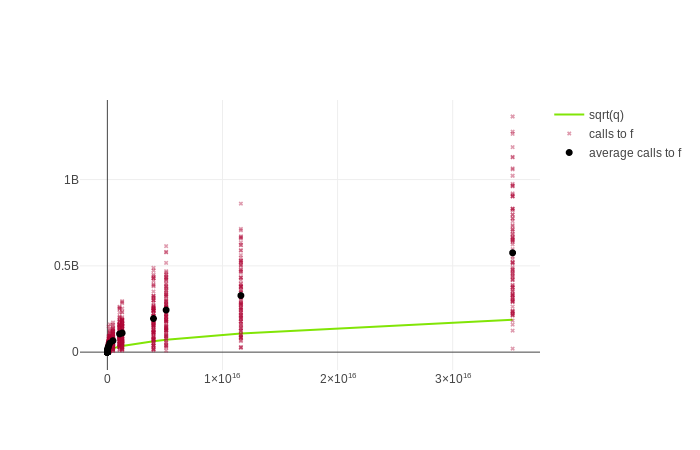
\includegraphics[scale=0.5]{images/iteration_r_adding_walks.png}
        \caption{Nombre d'appels à la fonction d'itération (r-adding walks) avant la détection d'une collision en fonction de la taille de $q$}
        \label{fig:r_adding_walks_iteration_results}
      \end{figure}

      Encore une fois, le graphe obtenu (figure \ref{fig:r_adding_walks_iteration_results}) confirme que la complexité de l'algorithme est en $\mathcal{O}(\sqrt{q})$.


    \section{Méthode des points distingués}
      \subsection{Théorie}
      Trouver un moyen de détecter une collision le plus rapidement possible après que celle-ci ait eu lieu est un autre problème important.  L'objectif est de limiter au maximum le nombre d'appels à la fonction d'itération avant d'obtenir une collision, tout en utilisant peu de mémoire. Plusieurs méthodes ont été développées ; parmi elles, celle des points distingués de Quisquater et Delescaille~\autocite[4]{pollard1} est considérée comme la plus efficace.

      On commence par choisir une propriété sur les éléments de $G$ qui soit facilement vérifiable - par exemple, avoir une écriture binaire se terminant par un certain nombre de $0$. Les éléments de $G$ satisfaisant cette propriété sont appelés les points distingués.

      On choisit un élément de $G$ de manière aléatoire et on lance la fonction d'itération dessus. Les appels à cette fonction s'arrêtent lorsqu'on a obtenu un point distingué. Celui-ci est alors stocké dans une table (on stocke également $a_i$ et $b_i$ tels que cet élément de $G$ s'écrit $g^{a_i} \cdot h^{b_i}$), et on choisit un autre élément de $G$ de manière aléatoire avant de réitérer le procédé. L'algorithme s'arrête lorsqu'on a trouvé deux points distingués égaux. Il y a fort à parier qu'on est parti de deux éléments différents de $G$ pour trouver ce point distingué, et que par conséquent on ait trouvé deux écritures différentes du point distingué en fonction de $g$ et $h$. On obtient donc des éléments $a_i$, $b_i$, $a_j$ et $b_j$ tels que $g^{a_i} \cdot h^{b_i} = g^{a_j} \cdot h^{b_j}$ avec $(a_i,b_i) \neq (a_j,b_j)$ et on peut résoudre le problème du logarithme discret.

      Pour que cette méthode fonctionne correctement, il faut choisir la propriété de telle sorte à ce que la table soit de taille manipulable. Cependant, si la propriété fixe quelques bits, alors ces bits n'ont pas besoin d'être stockés dans la table, ce qui permet des économies de mémoire (par exemple, si tous les points distingués se terminent par un même chiffre, inutile de le stocker dans la table). Si on note $\theta$ la fraction des éléments de $G$ satisfaisant la propriété des points distingués, alors l'algorithme doit terminer avec collision après environ $\sqrt{q\pi/2} + 1/\theta$ appels à la fonction d'itération. L'intérêt majeur de la méthode est qu'elle permet le traitement parallèle par plusieurs processeurs, ce qui permet des résultats encore meilleurs.

      % TODO
      \subsection{Implémentation}
      \subsection{Résultats}
      Toujours en utilisant le protocole défini dans le chapitre précédent (\ref{chapter2:protocole_de_mesure}), nous avons mesuré les performances de l'implémentation de la méthode des points distingués dans notre programme.

      \begin{figure}
        \center{}
        \includegraphics[scale=0.5]{images/distinguished_points.png}
        \caption{Nombre d'appels à la fonction d'itération (r-adding walks) avant la détection d'une collision selon la méthode des points distingués en fonction de la taille de $q$}
        \label{fig:r_adding_walks_and_distinguished_points_results}
      \end{figure}

      Le graphe obtenu (figure \ref{fig:r_adding_walks_and_distinguished_points_results}) met en évidence que la méthode des points distingués n'a pas changé la complexité de l'algorithme, toujours est en $\mathcal{O}(\sqrt{q})$.


    \section{Comparaison}
    Au final, nous avons implémenté deux fonctions d'itération différentes
    \begin{enumerate*}
      \item "basique" (telle que présentée dans le \textit{Handbook}~\autocite[107]{handbook})
      \item r-adding walks
    \end{enumerate*}
    , ainsi que deux méthodes de détection de collisions
    \begin{enumerate*}
      \item le lièvre et la tortue
      \item méthode des points distingués.
    \end{enumerate*}

    Ainsi, nous avons pu en mesurer les performances afin de pouvoir les comparer. Finalement, nous avons récolté des données pour les combinaisons suivantes :

    \begin{itemize}
      \item fonction d'itération basique et méthode du lièvre et de la tortue.
      \item r-adding walks et méthode du lièvre et de la tortue.
      \item r-adding walks et méthode des points distingués.
    \end{itemize}

    Dans la continuité de ce que nous avons présenté jusqu'à présent, nous avons rassemblé sur un même graphe (figure \ref{fig:comparatif}) les performances des différentes combinaisons de méthodes mesurées.

    \begin{figure}
      \center{}
      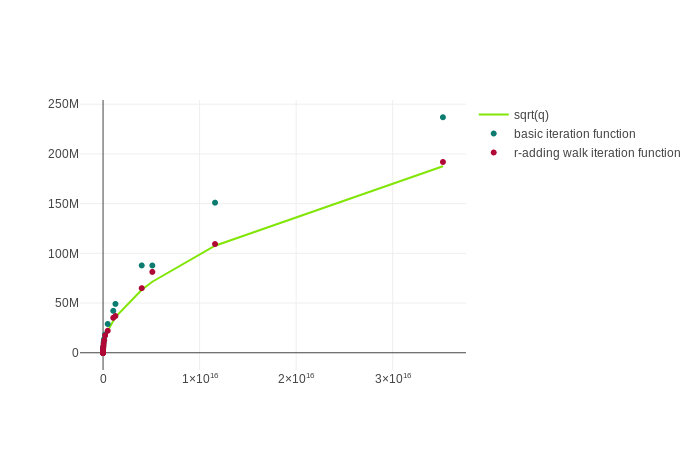
\includegraphics[scale=0.5]{images/comparaison_methodes.png}
      \caption{Nombre d'appels à la fonction d'itération selon les différentes implémentations avant la détection d'une collision en fonction de la taille de $q$}
      \label{fig:comparatif}
    \end{figure}

    On voit alors clairement que la combinaison des méthodes r-adding walks et des points distingués apporte une nette amélioration dans la résolution du problème sans pour autant en changer la complexité calculatoire, toujours en $\mathcal{O}(\sqrt{q})$.


    \section{Tag Tracing}
      \subsection{Présentation}
      Quand on applique la fonction d'itération des r-adding walks à un élément $x_i$ appartenant à $G$, on obtient un élément $x_{i+1}$ défini par $x_{i+1} = x_i M_{s(x_i)}$. Avec la méthode des points distingués, ce résultat est parfois stocké dans une table, ce qui nous amène à nous poser la question suivante~: étant donné qu'on ne stocke pas tous les éléments de la suite des $(x_i)_{i \ge 0}$, est-il vraiment nécessaire de les calculer à chaque fois ? Dans cette partie, nous décrirons une optimisation reposant sur cette idée.

      On commence par choisir deux petits entiers positifs $r$ et $l$. On fixe $S=\{0,\cdots,r-1\}$ et on construit $M=\{M_s = g^{m_s} h^{n_s}\}_{s \in S}$ comme pour la méthode des r-adding walks. On pose $M_l = (M\cup\{1\})^l$. C'est un tableau contenant l'ensemble des produits d'au plus $l$ éléments de $M$ listés avec les $a_i$ et $b_i$ de leur écriture $g^{a_i} h^{b_i}$.

      On fixe ensuite un ensemble $T$ avec trois fonctions~:

      $\begin{array}{lrcl}
        \tau : & G & \longrightarrow & T
      \end{array}$

      $\begin{array}{lrcl}
        \overline{\tau} : G \times M_l \longrightarrow & T \cup \{fail\}
      \end{array}$

      $\begin{array}{lrcl}
        \sigma : T \longrightarrow & S
      \end{array}$

      On définit également la fonction d'indexation $s$ et une autre fonction $\overline{s}$ de la façon suivante~:

      $\begin{array}{lrcl}
        s : & G & \longrightarrow & S \\
            & x & \longmapsto & \sigma \circ \tau (x)
      \end{array}$

      $\begin{array}{lrcl}
        \overline{s} : & G \times M_l & \longrightarrow & S \cup \{fail\} \\
                       & x & \longmapsto & \sigma \circ \overline{\tau} (x)
      \end{array}$

      On doit choisir $T$ et les fonctions $\tau$, $\overline{\tau}$ et $\sigma$ de sorte à ce que $s$ et $\overline{s}$ respectent quelques propriétés. Ainsi $s$ doit être surjective. De plus, si on regroupe les éléments de $G$ selon leur image par $s$, cette fonction doit diviser $G$ en une partition de $r$ sous-ensembles ayant environ la même taille. Si $\overline{s}(g,M) \in S$, alors on doit avoir $\overline{s}(g,M) = s(g M)$. On s'attend à ce que pour tout $M \in M_l$ et pour tout $g \in G$, calculer $\overline{s}(g,M)$ prenne moins de temps que de calculer $s(g,M)$, et on note le temps attendu par un calcul de $\overline{s}(g,M)$ par $|\overline{s}|$ quand $M \in M_l$.

      La fonction d'itération suit le même principe que celle des r-adding walks, mais dans notre cas la fonction d'indexation est $s = \sigma \circ \tau$. On choisit aléatoirement un élément $x_0 \in G$. Notre premier index est $s_0 = s(g_0)$. Comme pour la méthode des r-adding walks, on pose $x_1 = x_0 M_{s(x_0)}$. Cependant, on ne calcule pas $x_1$ mais $\overline{s}(x_0,M_{s(x_0)})$. Par définition, si le résultat appartient à $S$ alors il est égal à $s(x_0 M_{s(x_0)})$, c'est-à-dire $s(x_1) = s_1$.

      De même, $x_2 = x_1 M_{s_1} = x_0 M_{s_0} M_{s_1}$. Cependant, on ne calcule pas $x_2$ mais $\overline{s}(x_0,M_{s_0} M_{s_1})$ ($M_{s_0} M_{s_1}$ appartient à $M_l$, donc on peut le faire en temps $|\overline{s}|$). Si ce nombre appartient à $S$, alors il est égal à $s(x_0 M_{s_0} M_{s_1})$, c'est-à-dire $s_2$.

      On réitère le procédé jusqu'à calculer un $\overline{s}(x_0,M_{s_0} \cdots M_{s_k})$ qui n'appartient pas à $S$, ou jusqu'à arriver à $l$ itérations du procédé ci-dessus (au vu de la définition de $M_l$, cela signifie que lors de l'étape suivante le produit des $M_i$ n'appartiendrait pas à $M_l$). Quand un tel cas se produit, on calcule $x_{k+1} = x_0 M_{s_0} \cdots M_{s_k}$. Comme $M_{s_0} \cdots M_{s_k} \in M_l$, cela requiert une unique multiplication. On réitère alors le procédé en donnant à $x_{k+1}$ le rôle qu'avait $x_0$ jusqu'alors.

      On détecte une collision en utilisant la méthode des points distingués. Ici, un élément de $G$ doit satisfaire deux propriétés pour être un point distingué~:

      \begin{itemize}
        \item son écriture binaire se termine par un certain nombre de bits égaux à $0$.
        \item c'est un point $x_k$ tel que $\overline{s}(x_0,M_{s_0} \cdots M_{s_{k-1}})$ n'appartient pas à $S$.
      \end{itemize}

      La deuxième propriété assure que tous les potentiels points distingués sont calculés en suivant la méthode décrite plus haut (ce sont même les seuls éléments de la suite $(x_i)_{i \ge 0}$ que l'on calcule). On peut donc se permettre de ne vérifier la première propriété que parmi ces éléments, et utiliser $\overline{s}$ et la méthode décrite ci-dessus pour ne pas avoir à calculer tous les autres éléments (qui ne vérifient de toute façon pas la deuxième propriété et ne sont donc pas des points distingués).


    \subsection{Application}
    Soient $p$ un nombre premier et $G$ le sous-groupe cyclique d'ordre $q$ premier de $(\mathbb{Z}/p\mathbb{Z})^*$. Commençons par donner des contraintes pour le choix des entiers $l$ et $r$ (pour rappels, $S = \{0,1,\cdots,r-1\}$, $M=\{M_s = g^{m_s} h^{n_s}\}_{s \in S}$, et on pose $M_l = (M\cup\{1\})^l$).

    $M_l$ a une taille d'au plus $\binom{l+r}{r}$. En effet, chaque élément de $M_l$ est obtenu en choisissant $l$ éléments de $M\cup\{1\}$ (on peut prendre plusieurs fois le même élément) et en les multipliant entre eux (si un élément de $M_l$ est le produit de moins de $l$ éléments de $M = \{M_s = g^{m_s} h^{n_s}\}_{s \in S}$, alors comme $1$ appartient à $M\cup\{1\}$, on peut toujours l'écrire comme produit de $l$ éléments de $M\cup\{1\}$). Par conséquent, le nombre d'éléments de $M_l$ correspond au nombre de combinaisons avec répétitions de $l$ éléments parmi $r + 1$ éléments ($M_l = (M\cup\{1\})^l$ et $M$ est de taille $r$).

    Le nombre de combinaisons avec répétitions de $p$ éléments parmi $n$ est $\binom{n+p-1}{p}$ ou encore $\binom{n+p-1}{n-1}$. La deuxième formule donne le résultat.

    Montrons à présent que l'ensemble $M_l$ peut être construit en $\binom{l+r}{r} - r - 1$ multiplications dans $G$.

    On crée un arbre de cette façon~:

    \begin{itemize}
      \item l'arbre a une profondeur de $l$.
      \item de chaque noeud partent très exactement $r$ branches, qui ont toutes un label différent (allant de $0$ à $r - 1$).
      \item on donne au noeud se situant à la racine de l'arbre le label $1$.
      \item le label des autres noeuds est l'élément de $M_l$ correspondant aux produits des éléments de $M$ associés aux labels des branches situées entre ce noeud et le noeud racine.
    \end{itemize}

    Dans cette structure, on trouve un même élément de $M_l$ plusieurs fois. Pour construire $M_l$, il suffit de collecter les labels des noeuds de l'arbre correspondant à des chemins dont les branches ont un label décroissant. On a prouvé qu'il y a $\binom{l+r}{r}$ noeuds différents dans les branches retenues. Or parmi ces noeuds il y a~:

    \begin{itemize}
      \item un noeud ayant pour label $1$.
      \item $r$ noeuds ayant pour labels les différents éléments de $M = \{M_s = g^{m_s} h^{n_s}\}_{s \in S}$, que l'on a déjà calculés.
      \item tous les autres noeuds, qui sont des produits d'éléments de $M$. Il y en a $\binom{l+r}{r} - r - 1$.
    \end{itemize}

    Donc on a besoin de $\binom{l+r}{r} - r - 1$ multiplications dans $G$ pour construire $M_l$.

    Il faut donc choisir les entiers $l$ et $r$ de manière à ce que la table des $M_l$ ait une taille manipulable et que le calcul des éléments de $M_l$ se fasse en un nombre de multiplications négligeable par rapport aux appels de la fonction d'itération.

    On construit l'ensemble $T$ ainsi~: on choisit un entier positif $b$ et on pose $t = rb$. On pose ensuite $T = \{0,1,\cdots,t-1\}$. On choisit un petit entier $\epsilon$ et on pose $d = \lceil\log_\epsilon(p)\rceil$. On choisit ensuite un entier $\omega'$ tel que $\omega' \ge d(\epsilon - 1) + 1$ et on pose $\omega = t\omega'$. On doit avoir $\omega < p^{1/3}$. On prouvera plus tard que ces contraintes permettent d'assurer que Tag Tracing fonctionne avec les fonctions que nous nous apprêtons à définir. Cependant, les choix optimaux pour ces paramètres sont variables. Ils dépendent en effet de facteurs tels que la taille de $p$, les ressources disponibles et la vitesse à laquelle la machine utilisée est capable de multiplier de grands entiers.

    Définissons à présent les fonctions~:

    $\begin{array}{lrcl}
      \tau : G \longrightarrow & T
    \end{array}$

    $\begin{array}{lrcl}
      \overline{\tau} : G \times M_l \longrightarrow & T \cup \{fail\}
    \end{array}$

    $\begin{array}{lrcl}
      \sigma : T \longrightarrow & S
    \end{array}$

    On pose $\sigma(x) = \lfloor x/b \rfloor$. On doit avoir $\sigma : T \longrightarrow S$. Soit $x \in T = \{0,1,\cdots,t-1\}$ On a $t = rb$, donc $0 \leq x < rb$, ce qui implique $0 \leq x/b < r$ et donc $0 \leq \lfloor x/b \rfloor < r$ et comme c'est un entier on a bien $\sigma(x) \in S=\{0,\cdots,r-1\}$. De plus, chaque élément de $S$ a au moins un antécédent par $\sigma$, donc la fonction est surjective.

    On choisit un entier $B$ satisfaisant les propriétés suivantes~:  $B > p^{2/3}$ et $0 \leq \omega B - p < B^{1/2}$. Il suffit par exemple de poser $B = \lceil p/\omega \rceil$. En effet, comme $w < p^{1/3}$, on a $p/\omega > p/p^{1/3} = p^{2/3}$. On pose ensuite $\tau(x) = \lfloor \frac{x\mod p}{\omega' B} \rfloor$.

    On doit avoir $\tau : G \longrightarrow T$. On a choisi $B$ de sorte à ce que $0 \leq \omega B - p$ et on a posé $\omega = t\omega'$. On a donc $0 \leq t \omega' B - p$, ce qui implique $\frac{p}{\omega' B} \leq t$. Par conséquent, $\frac{p-1}{\omega' B} < t$. Or $x\mod p \in \{0,1,\cdots,p-1\}$, donc $0 \leq \frac{x\mod p}{\omega' B} < t$ pour tout $x \in G$, et on a bien $\tau(x) \in T$.

    On a donc défini la fonction d'indexation $s = \sigma \circ \tau : G \longrightarrow S$. $s$ est bien surjective car $\sigma$ et $\tau$ le sont. La deuxième propriété que doit satisfaire $s$ est de diviser $G$ en une partition de $r$ sous-ensembles ayant environ la même taille si on regroupe les éléments de $G$ selon leur image par $s$. C'est une propriété appelée être uniforme par la pré-image. On peut le montrer en prouvant que $\tau$ est uniforme par la pré-image.

    Il nous reste à définir $\overline{\tau}$. Soient $x$ et $y$ appartenant à $(\mathbb{Z}/p\mathbb{Z})^*$. On a $d = \lceil\log_\epsilon(p)\rceil$, donc on peut écrire $x$ en base $\epsilon$~:

    $$ \sum_{i=0}^{d-1} x_i \epsilon^i \text{ avec $0 \leq x_i < \epsilon$} $$

    Pour tout entier $i$ appartenant à $\{0,1,\cdots,d-1\}$, on peut trouver des éléments $\hat{y_i}$ et $\tilde{y_i}$ avec $0 \leq \hat{y_i} \leq \frac{p-1}{B} < \omega$ et $0 \leq \tilde{y_i} < B$ tels que $\epsilon^i y\mod p = \hat{y_i} B + \tilde{y_i}$.

    On définit $\overline{\overline{\tau}} : G \times M_l \longrightarrow T \cup \{fail\}$ par~:

    $$\overline{\overline{\tau}}(x,y) = \lfloor \frac{\sum_{i=0}^{d-1} x_i \hat{y_i}\mod \omega}{\omega'} \rfloor$$

    Montrons que pour tout $x$ et $y$ de $(\mathbb{Z}/p\mathbb{Z})^*$, on a $\tau(xy) = \overline{\overline{\tau}}(x,y)$ ou $\tau(xy) = \overline{\overline{\tau}}(x,y) + 1$ si $\overline{\overline{\tau}}(x,y) \neq t - 1$.

    On trouve $a_0$, $a_1$ et $a_2$ tels que~:

    $$ \sum_{i=0}^{d-1} x_i \hat{y_i} = a_2\omega + a_1\omega' + a_0 $$

    Pour cela, on divise $\sum_{i=0}^{d-1} x_i \hat{y_i}$ par $\omega$ ; le quotient de cette division est le coefficient $a_0$, le reste correspond à $a_1\omega' + a_0$. Pour trouver $a_1$ et $a_0$, il suffit donc de calculer le quotient et le reste dans la division de $a_1\omega' + a_0$ par $\omega'$.

    On a $\overline{\overline{\tau}}(x,y) = a_1$. En effet, on a~:

    \begin{align*}
    \overline{\overline{\tau}}(x,y) &= \lfloor \frac{\sum_{i=0}^{d-1} x_i \hat{y_i}\mod \omega}{\omega'} \rfloor \\
                                    &= \lfloor \frac{a_2\omega + a_1\omega' + a_0\mod \omega}{\omega'} \rfloor \\
                                    &= \lfloor \frac{a_1\omega' + a_0\mod \omega}{\omega'} \rfloor
    \end{align*}

    Or $a_1\omega' + a_0$ est le reste dans la division euclidienne de $a_2\omega + a_1\omega' + a_0$ par $\omega$, donc par définition $0 \leq a_1\omega' + a_0 <  \omega$, par conséquent $\lfloor \frac{a_1\omega' + a_0\mod \omega}{\omega'} \rfloor = \lfloor \frac{a_1\omega' + a_0}{\omega'} \rfloor$. Donc on a $\overline{\overline{\tau}}(x,y) = \lfloor a_1 + a_0/\omega' \rfloor$. Or $a_0$ est le reste dans la division euclidienne de $a_1\omega' + a_0$ par $\omega'$, donc $0 \leq a_0 < \omega'$, donc $0 \leq a_0/\omega' < 1$, et comme $a_1$ entier on a $\lfloor a_1 + a_0/\omega' \rfloor = a_1$.

    $\sum_{i=0}^{d-1} x_i \hat{y_i} \leq d \text{\ max }\{x_i\} \hat{y_i} \leq d(\epsilon - 1)(\omega - 1)$. Donc $a_2 \leq \frac{d(\epsilon - 1)(\omega - 1)}{\omega}$. On a ainsi~:

    $$a_2 \leq \frac{d(\epsilon - 1)(\omega - 1)}{\omega} < d(\epsilon - 1) < \omega' < \omega < B^{1/2} $$

    Par ailleurs, $xy = \sum_{i=0}^{d-1} x_i \epsilon^i y$. Comme $\epsilon^i y\mod p = \hat{y_i} B + \tilde{y_i}$, on a~:

    \begin{align*}
        xy &\equiv B(\sum_{i=0}^{d-1} x_i \hat{y_i}) + \sum_{i=0}^{d-1} x_i \tilde{y_i} \text{\ mod} p \\
           &\equiv B a_2\omega + B a_1\omega' + B a_0 + \sum_{i=0}^{d-1} x_i \tilde{y_i} \text{\ mod} p
    \end{align*}

    $-a_2 p \equiv 0 \text{\ mod} p$, donc on peut écrire $xy \equiv a_2(B\omega - p) + B a_1\omega' + B a_0 + \sum_{i=0}^{d-1} x_i \tilde{y_i} \text{\ mod} p$. Concentrons-nous sur $a_2(B\omega - p) + B a_0 + \sum_{i=0}^{d-1} x_i \tilde{y_i}$ et majorons ce nombre.

    $a_0$ est le reste dans la division euclidienne de $a_1\omega' + a_0$ par $\omega'$, donc $0 \leq a_0 < \omega'$. De plus on a montré précédemment que $a_2 < B^{1/2}$ et on a également $B\omega - p < B^{1/2}$. Enfin, $\tilde{y_i} \leq B - 1$ et $\sum_{i=0}^{d-1} x_i \leq d \text{\ max $\{x_i\}$} \leq d(\epsilon - 1)$ car $x_i \leq \epsilon - 1$. On peut donc en conclure~:

    \begin{align*}
    a_2(B\omega - p) + B a_0 + \sum_{i=0}^{d-1} x_i \tilde{y_i} &< B(\omega' - 1) + B^{1/2}B^{1/2} + d(\epsilon - 1)(B - 1) \\
                            &< B\omega' + B^{1/2}B^{1/2} + d(\epsilon - 1)(B - 1) \\
                            &< B\omega' + d(\epsilon - 1)(B - 1) \\
                            &< B\omega' + \omega'(B - 1) \text{\ car $d(\epsilon - 1) < \omega'$} \\
                            &< 2B\omega' - B
    \end{align*}

    Supposons que $a_1 = \overline{\overline{\tau}}(x,y)$ est strictement inférieur à $t - 1$. On a donc~:

    \begin{align*}
    a_2(B\omega - p) + B a_1\omega' + B a_0 + \sum_{i=0}^{d-1} x_i \tilde{y_i} \text{\ mod} p &< (t - 2)B\omega' + 2B\omega' - B \\
                          &< tB\omega' - B \\
                          &< B\omega - B \text{\ car $\omega = t\omega'$} \\
                          &< p \text{\ car $B = \lceil p/\omega \rceil$}
    \end{align*}

    Donc $xy \text{\ mod } p = B a_1\omega' + a_2(B\omega - p) + B a_0 + \sum_{i=0}^{d-1} x_i \tilde{y_i}$. De plus, on a montré que $a_2(B\omega - p) + B a_0 + \sum_{i=0}^{d-1} x_i \tilde{y_i} < 2B\omega' - B < 2B\omega'$. Cette quantité est également positive, donc le quotient de la division euclidienne de $xy$ par $B\omega'$ est $a_1$ ou $a_1 + 1$. Or $\tau(xy) = \lfloor \frac{xy\mod p}{\omega' B} \rfloor$ et $\overline{\overline{\tau}}(x,y) = a_1$, donc on a terminé la preuve.

    On peut alors définir $\overline{\tau}$ de la manière suivante~:

    \begin{align*}
      \overline{\tau}(g,M) =
      \begin{cases}
        \text{\ fail } & \text{si } \overline{\overline{\tau}}(g,M) \text{\ mod $b$ est $b - 1$ ou $b - 2$} \\
        \overline{\overline{\tau}}(g,M)  & \text{ sinon}
      \end{cases}
    \end{align*}

     On a ainsi défini la fonction $\overline{s} = \sigma \circ \overline{\tau}$.  Il faut maintenant montrer que si $\overline{\tau}(x,M) \in T$ (et donc $\overline{s}(x,M) \in S$), on a $s(xM)=\overline{s}(x,M)$ et $\tau(xM) \text{\ mod } b \neq b - 1$.

     $\overline{\tau}(x,M) \in T$ quand $\overline{\overline{\tau}}(x,M) \neq b - 1$ et $\overline{\overline{\tau}}(x,M) \neq b - 2$. Or comme $t = rb$, on a $t - 1 \text{\ mod } b = b - 1$. Donc on n'a pas $\overline{\overline{\tau}}(x,M) = t - 1$. On a prouvé précédemment que dans ce cas $\tau(xM) = \overline{\overline{\tau}}(x,M)$ ou $\overline{\overline{\tau}}(x,M) + 1$.

     Comme $\overline{\overline{\tau}}(x,M) \neq b - 1$ et $\overline{\overline{\tau}}(x,M) \neq b - 2$, on a $\tau(xM) \text{\ mod } b \neq b - 1$. De plus, $\overline{\tau}(x,M) = \overline{\overline{\tau}}(x,M)$, donc $\overline{\tau}(x,M) \text{\ mod } b \neq b - 1$. Par conséquent~:

     $$\lfloor \frac{\overline{\tau}(x,M)}{b} \rfloor = \lfloor \frac{\overline{\tau}(x,M) + 1}{b} \rfloor$$

     On a $\sigma(x) = \lfloor x/b \rfloor$ et $s= \sigma \circ \tau$. Donc $s(xM) = \overline{s}(x,M)$.
